\documentclass{article}
%\setkomafont{disposition}{\normalfont\bfseries}

\usepackage{listings}
\usepackage{color}
\usepackage{amsmath}
\usepackage{graphicx}
\usepackage{float}
%\usepackage[toc,page]{appendix}
\usepackage{caption}
\usepackage[margin=1.25in]{geometry}
%\usepackage{apacite}
\usepackage{url}
\usepackage{appendix}
\usepackage{pdfpages}
%\usepackage[demo]{graphicx}
\usepackage{caption}
\usepackage{subcaption}
\usepackage{rotating}
\usepackage{tikz}
\usepackage{hhline}
\usepackage[hidelinks]{hyperref}


\tikzset{%
	block/.style    = {draw, thick, rectangle, minimum height = 3em,
		minimum width = 3em},
	sum/.style      = {draw, circle, node distance = 2cm,fill=blue!20}, % Adder
	input/.style    = {coordinate}, % Input
	output/.style   = {coordinate} % Output
}
% Defining string as labels of certain blocks.
\newcommand{\suma}{\Large$+$}
\newcommand{\inte}{$\displaystyle \int$}
\newcommand{\derv}{\huge$\frac{d}{dt}$}


\usepackage{fancyhdr}
\pagestyle{fancy}
\fancyhf{}
\lhead{2127147}
\rhead{Subtractive Synth}
\rfoot{Page \thepage}



\title{\textbf{A Subtractive Synthesiser \\ using C++, Python \& SWIG\\
\large Audio Programming and Signal Processing 4 }}

\date{}
\author{Jamie Brown}

\begin{document}
	\vspace{100mm}
	\maketitle
	\thispagestyle{fancy}
	\pagenumbering{arabic}
\centering
\begin{abstract}
	Realtime audio synthesis requires fast computations in order to provide low latency for the user. Using a modular, object orientated approach, a subtractive synthesizer has been designed using the Python alongside a C++ module that has been interfaced using SWIG. 
\end{abstract}
\vspace{2cm}
\includegraphics[width=0.4\linewidth]{window.png} 
\pagebreak
\flushleft
\section{Introduction}
As this program is rather complex, it's useful to develop an abstracted, modular design considering the roles of desired modules (classes). What is required in order to develop a functioning software synthesiser?

\begin{enumerate}
	\item A source of synthesised sound (additive, subtractive, stochatic etc.)
	\item An audio buffer
	\item A graphical interface for the user
	\item A module to handle incoming MIDI events
	\item A module to route the input data from the GUI and MIDI
\end{enumerate} 
A modular design really necessates an object oriented approach so we'll use Python to develop points two to five as we can use pyQtMultimedia, pyQtWidgets and mido  to make the programming easier than C++. Point one (sound source) is a little trickier as this is going to require speed, we'll use C++ to code this.
\section{Resonator}
One way to synthesise a tone is using subtractive synthesis. 
This usually involves generating noise and band pass filtering around the centre frequency to generate the tone. 
A common method of doing this is by using a second order infinite impulse response filter (IIR).
Firstly, let's look at the transfer function for a resonator with a centre frequncy around $f_0$ in the Z domain:
\begin{equation}
H(Z)=\frac{1}{1-2rcos\theta Z^{-1}+r^2Z^{-2}}
\end{equation}
From this we can derive a data flow diagram. We don't need to use a standard biquad form as the feed-forward coefficiant(the numerator) in this case is 1  so the output of the filter is simply the output of the first summing junction. A larger $r$, as we approach the edge of the unit circle, will result in a narrower, taller pass band due to the longer impulse response. This would result in a less noisy, more defined sounding tone as the pass band draws in around the centre frequency. We're going to design our resonator to have a variable r, by varying the \textit{quality-factor}.


\tikzstyle{block} = [draw,fill=blue!20,minimum size=2em]
% diameter of semicircle used to indicate that two lines are not connected
\def\radius{.7mm} 
\tikzstyle{branch}=[fill,shape=circle,minimum size=3pt,inner sep=0pt]
\begin{figure}[H]
	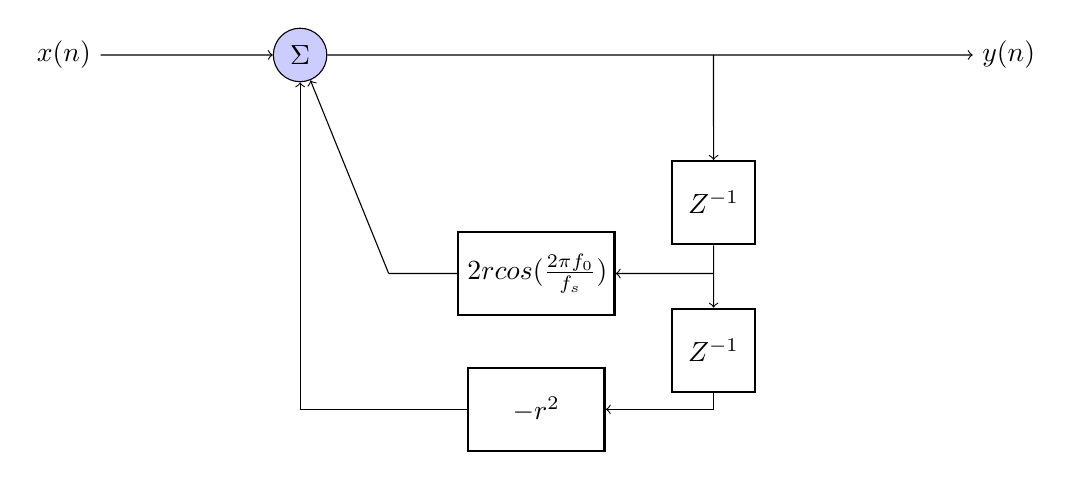
\begin{tikzpicture}[node distance=2cm>=latex',scale=1.5]
	
	\node[sum] at (3,-1) (block1) {$\Sigma$};
	\node[block][text width=1.75cm,align=center] at (5,-2.85) (cos) {$2rcos(\frac{2\pi f_0}{f_s})$};
	\node[block][text width=1.5cm,align=center] at (5,-4) (r) {$-r^2$};
	\node[block] at (6.5,-2.25) (z1) {$Z^{-1}$};
	\node[block] at (6.5,-3.5) (z2) {$Z^{-1}$};
	\node[input] at (2,-2) (block11) {ADC$_channel1$};
	%\node[block][text width=1.5cm,align=center] at (6.5,-1) (block5) {$F_{static}$};
%	\node[block] at (8.25,-4.5) (block8) {$\frac{1}{t_{s}}$};
%	\node[sum] at (8.25,-1) (block6) {$\Sigma$};  
%	\node[sum] at (6.75,-4.5) (block9) {$\Sigma$};    
%	\node[block] at (6.025,-3.125) (block10) {$-2$};
%	\node at (2,-2.75) (input2) {ADC$_2$};
	\node at (1,-1) (input1) {$x(n)$};
	\node at (9,-1) (input3) {$y(n)$};
	
	\draw[->] (input1) -- (block1);
	\draw[->] (block1) -- (input3);
	\draw[->] (r) -| (block1);
	\draw[-] (cos) -- (3.75,-2.85);
	\draw[->] (3.75,-2.85) --(block1);
	\draw[->] (6.5,-1) -- (z1);
	\draw[->] (z1) -- (z2);
	\draw[->] (6.5,-2.85) -- (cos);
	\draw[->] (z2) |- (r);
	
	
	\end{tikzpicture}
	\caption{Resonator Data Flow Diagram}
\end{figure}

\pagebreak
\subsection{C++}
The resonator module has one method \textit{filter{}}. It's sole purpose is to generate one sample from a random floating point and is designed to take in a value for the centre frequency, the desired quality factor (Q) and the sampling frequency. It has to know what the sampling rate is because the frequency needs to be normalised before the module can correctly calculate the first coefficients. The following equation is used to evaluate r in relation to the Q-factor:
\begin{equation}
r=1-sin({\frac{\omega_0}{Q}})
\end{equation}  
We now need two buffers, one for each delay step, to store the previous samples to complete the computation. These need to be initialised in the constructor as we don't want them to be overwritten every time the \textit{filter{}} method gets called as that would defeat the purpose. 
\begin{figure}[H]

\begin{lstlisting}[language=C++]
Resonator::Resonator(float f, float q, int SAMPLE_RATE) :
w(2*atan(1)*4*(f/SAMPLE_RATE)),r(1-sin(w/q)),a1(-2*r*cos(w))
,a2(pow(r,2)),buffer1(0),buffer2(0),x(f)
{
}

\end{lstlisting}
\caption{Resonator.cxx constructor}
\end{figure}

The \textit{filter()} method is an exact implementation of the data flow diagram seen in figure 1. We start by generating a random floating point between 0 and 1, equivalent to $x(n)$. The summing junction is equivalent to `acc\_input' which is written to `buffer1' after computation. Each value is shifted along to the next buffer to store them for when the method is next called, this is equivalent to the two delay blocks in figure 1. The returned value `acc\_input' is equivalent to y(n).
\begin{figure}[H]
	\begin{lstlisting}[language=C++]
float Resonator::filter(){
	float v=static_cast <float> (rand())/static_cast <float> (RAND_MAX);
	float acc_input=v-buffer1*a1-buffer2*a2;	
	buffer2=buffer1;
	buffer1=acc_input;
	return acc_input;
}	
	\end{lstlisting}
	\caption{Resonator.cxx filter() method}
\end{figure}
All constructor variables and methods are initialised in the header file which is included in the appendix.
\subsection{Generating the Python Module}
The differences between the two languages are numerous, most notably related to memory allocation and types. To generate a resonator module in Python we can use the Simple Wrapper Interface Generator (SWIG) to generate wrapper code that can be linked to the C++ object files. However, there are a few things that need to be taken care of first. 
\subsubsection{Interface File}
An interface file needs to be made in order to parse the appropriate files to SWIG and let it know what module needs to be made. In this case the interface file is very simple:
\begin{figure}[H]
	\begin{lstlisting}[language=c]
%module Resonator

%{
#define SWIG_FILE_WITH_INIT
#include "Resonator.h"
%}

%include "Resonator.h"
 
	\end{lstlisting}
	\caption{Interface file for the resonator: \textit{Resonator.i}}
\end{figure} 
\subsubsection{makefile}
Now that an interface file has been created, it's time to actually compile the C++ program! The easiest way to do this and minimise frustration during future debugging is to write a make file that compiles the necessary files and also assigns dependicies. This means that if a file, such as the header file, is altered then when \textbf{make} is executed, only the necessary files are rebuilt. This example line of code from my makefile shows that the target object file (Resonator.o) is dependent on the C++ file (Resonator.cxx), if I don't modify Resonator.cxx then \textbf{make} won't bother executing the system command on the second line because it doesn't need to:
\begin{figure}[H]
\begin{lstlisting}[language=make]
Resonator.o: Resonator.cxx
	g++ -fPIC -c Resonator.cxx 
\end{lstlisting}
\caption{An example of a dependancy in the makefile}
\end{figure}
Another really handy use of the makefile for this program is that the command to generate the wrapper code from SWIG can be executed in the file itself. In this case, the target is the python file and it's dependancy is the interface file. The entire makefile is included in the appendix.
\begin{figure}[H]
	\begin{lstlisting}[language=make]
Resonator.py: Resonator.i
	swig -c++ -python Resonator.i 
	\end{lstlisting}
	\caption{Using SWIG to generate wrapper code in a makefile}
\end{figure}


Implementing our resonator in Python is as simple as importing any other shared object. I have imported it as \textbf{ResC} simply because I made a prototype resonator in Python for testing/debugging purposes, under the same name, so it is helpful to make it very clear that this module is the C++ version.
 \begin{figure}[H]
 	\begin{lstlisting}[language=python]
import Resonator as ResC
 	\end{lstlisting}
 	\caption{Importing a shared object into Python}
 	\end{figure}
 
\section{The Generator Object} 
\subsection{Audio Buffers}
A \textbf{Generator} object is used to call instances of the resonator and handle the synthesised audio in managable amounts of samples. It handles the resonator audio by supplying a chunk size of audio, `NO\_OF\_SAMPLES', which is the length of the buffer. The Generator is a subclass of the QIODevice module, this means that it inherits all the same attributes and methods as a QIODevice.

 \begin{figure}[H]
	\begin{lstlisting}[language=python]
class Generator(QIODevice):
SAMPLES_PER_READ=1024
def __init__(self,format,parent=None):
	self.format=format
	QIODevice.__init__(self,parent)
	self.data=QByteArray()
	\end{lstlisting}
	\caption{The generator constructor}
\end{figure}

The QIODevice needs a method \textit{start()} which has an attribute \textit{open()}. This simply indicates that the Generator is ready upon instantiation and is set as read-only:

 \begin{figure}[H]
	\begin{lstlisting}[language=python]
    def start(self):
		self.open(QIODevice.ReadOnly)

	\end{lstlisting}
	\caption{The \textit{start()} method}
\end{figure}
\subsection{Using the Resonator}
We want to create an instance of a Resonator when a new note is pressed. This can be done using a pyqtslot that passes a value when a `note-on' MIDI message is received, this is expained in further detail later. An incoming MIDI note value is converted to the desired frequency and passed to the new instance of the resonator:
 \begin{figure}[H]
	\begin{lstlisting}[language=python]
	@pyqtSlot(int)
	def noteOn(self,d):	
		self.state=1 
		f=(2**((d-69)/12))*440
		self.resonator=ResC.Resonator(f,self.q,SAMPLE_RATE)
	\end{lstlisting}
	\caption{pyqtSlot for generator when a `note\_on' message is received}
\end{figure}
\pagebreak
The audio is generated using the \textit{generate()} method. It creates an array with number of elements equal to the specified chunk size and writes samples to each entry by calling the resonator's \textit{filter()} method. The array is multiplied by a velocity scaling factor, volume scaling factor and on/off state. It is converted from floating point to 16-bit integer arithmetic for the QIODevice:
 \begin{figure}[H]
	\begin{lstlisting}[language=python]
    def generate(self,NO_OF_SAMPLES):
		tone=np.zeros(NO_OF_SAMPLES)
		for i in range(len(tone)):           
			tone[i]=self.resonator.filter()
		tone=(self.vel*50*tone*self.state*self.vol).astype(np.int16)	
	return tone.tostring()
	\end{lstlisting}
	\caption{The \textit{generate()} method}
\end{figure}
\subsection{How does Qt know when to read?}
A \textit{readData()} method has to be included so that Qt's executive reads samples to the output stream at the correct point depending on the specified chunk size:
 \begin{figure}[H]
	\begin{lstlisting}[language=python]
    def readData(self,bytes):
		if bytes>2*Generator.SAMPLES_PER_READ:
			bytes=2*Generator.SAMPLES_PER_READ
		return self.generate(bytes//2)
	\end{lstlisting}
	\caption{The \textit{readData()} method}
\end{figure}


\pagebreak
\section{MIDI}
A synthesiser is no use unless you can play it with a keyboard! Well that's not strictly true, you can play them with knobs, potentiometers, patch cables etc...but that doesn't change the fact that these signals have to digitally interfaced somehow and the defacto standard is MIDI.

\medskip I'm going to make an object that reads the MIDI ports and sends the appropriate messages depending on how a note is pressed. Firstly, we need a bit of backend software to get the MIDI up and running. 
\subsection{Rtmidi}
This MIDI backend is ideal because it's so widely used. Another advantage is that virtual ports can be created so that MIDI messages can be passed across threads, this will come in very useful later. This could also be very useful if you wanted to control some outboard hardware by outputting MIDI for instance. The following example uses the ALSA API as I'm running this on a LINUX machine.

 \begin{figure}[H]
	\begin{lstlisting}[language=python]
	def __init__(self):
		QObject.__init__(self)
		mido.set_backend(
		 'mido.backends.rtmidi/LINUX_ALSA'
		  )
	\end{lstlisting}
	\caption{Configuring the MIDI backend}
\end{figure}
\subsection{mido}
\textbf{mido} is an easy to use library of Python objects for MIDI programming. Using the following code, MIDI messages can be read and emitted to pyqt signals. A writeable MIDI client will be created under ALSA which we can use to connect a hardware controller of our choice. I've chosen to print out messages that I thought would be of use in testing the ports: the velocity of each note and whether it was a \textit{note-on} or \textit{note off}. 
 \begin{figure}[H]
	\begin{lstlisting}[language=python]
	with mido.open_input(
		'pipes',
		virtual=True
		) as mip:
		for mmsg in mip:
			print(mmsg.type)
			print(mmsg.velocity) 
	\end{lstlisting}
	\caption{Opening virtual ports and printing MIDI messages}
\end{figure}
	
\pagebreak
\subsection{MIDI Messages \& Routing}
With this we can generate signals for other modules or threads in the program in order to control certain parameters. I'm mostly interested in three of these: \textit{note-on}, \textit{note-off} and \textit{velocity}. In most conventional applications, the instrument should , to some extent, stop making a sound after the keys are released. We therefore need to send two signals to deal with this, I'll generate these based on the note's state using a standard \textit{if/else} clause. I'll also emit a signal containing the note's velocity:

 \begin{figure}[H]
	\begin{lstlisting}[language=python]
	if mmsg.type==`note_on':
		self.noteOn.emit(mmsg.note)
	elif mmsg.type==`note_off':
		self.noteOff.emit(mmsg.note)
	self.noteVelocity.emit(mmsg.velocity) 
	\end{lstlisting}
	\caption{Emitting MIDI messages through virtual ports}
\end{figure}

Lastly, the ports need to be initialised as methods:
 \begin{figure}[H]
	\begin{lstlisting}[language=python]
	class MidiPortReader(QObject):
		noteOn=pyqtSignal(int)
		noteVelocity=pyqtSignal(int)
		noteOff=pyqtSignal(int) 
	\end{lstlisting}
	\caption{Initialising virtual MIDI ports}
\end{figure}
These are now ready to be received as slots in other threads. It's worth bearing in mind that not all MIDI keyboards will send the same MIDI messages; many will in fact not send a \textit{note-off} and instead will send a second \textit{note-on} with a velocity of zero. I've accounted for this as each buffer gets multiplied by the velocity which is a float scaled from zero to one. 

\pagebreak
\section{GUI}
As stated in the introduction, we need a user interface for the instrument so that `uncomputery' folk can use it. As much as I'd delight in programming a command line driven UI for the synthesiser, it isn't exactly commercially viable or useful to most musicians. Alas, I have devised a somewhat minimalist GUI using QtGui and QtWidgets.
\subsection{Making the Clicky Things}
Buttons, sliders and labels like most things, have to be initialised to bring them into existence. Most of these objects have attributes that you can use to modify to get it looking how you want or outputting a certain scale of data. This is all done in a method called \textit{create\_UI} the  purpose of which is somewhat self-explanatory. The following few lines of code set up the volume slider and its corresponding label. The \textit{volumeSlider} is prefaced with \textit{self} because we're going to use it to send volume data through a virtual port:
 \begin{figure}[H]
	\begin{lstlisting}[language=python]
	volLabel=QLabel()
	volLabel.setText("Volume")
	self.volumeSlider=QSlider(Qt.Horizontal)
	#SET SLIDER SCALE 0-100
	self.volumeSlider.setMinimum(0)
	self.volumeSlider.setMaximum(100)) 
	\end{lstlisting}
	\caption{Initialising the volume slider}

\end{figure}	
\subsection{The Window Layout}
A total vertical layout is made alongside several horizontal layouts containing the sliders and their labels. These horizontal layouts are  arranged to fit into the overall vertical layout one by one. Here is an example of setting the vertical layout and superimposing the layout containing the Q-factor slider: 
 \begin{figure}[H]
	\begin{lstlisting}[language=python]
	vLayout=QVBoxLayout(self)
	h2Layout=QHBoxLayout()
	h2Layout.addWidget(qfacLabel)
	h2Layout.addStretch(1)
	h2Layout.addWidget(self.qfacSlider)
	\end{lstlisting}
	\caption{Initialising the volume slider}
	
\end{figure}
\pagebreak
\subsection{Quit Button}
The quit button is set to terminate the program when clicked by connecting it to its attribute \textit{quitClicked} using the following line of code in the \textit{create\_UI()} method: 
 \begin{figure}[H]
	\begin{lstlisting}[language=python]
       self.quitButton.clicked.connect(
       self.quitClicked
	)
	\end{lstlisting}
	\caption{Connecting the quit button}
	
\end{figure}
 
\subsection{Embedded Image}
Raster images of type .jpg or .png can be implemented in the GUI using \textit{QPixmap()}. I put a picture of David Lynch playing a synthesiser in the main window because David Lynch is cool.

 \begin{figure}[H]
	\begin{lstlisting}[language=python]
	    pixmap=QPixmap()
	    pixmap.load('lynch2.jpeg')
	    pixmap=pixmap.scaledToWidth(200)
	    self.lynch.setPixmap(pixmap)
	\end{lstlisting}
	\caption{Embedding a photograph of critically acclaimed filmmaker and musician David Lynch playing a synthesiser onto the GUI}
	
\end{figure}
 \pagebreak
 
 
\section{The Window Object}
This class contains the audio formatting, thread connections and GUI method. In a sense this is the central interface for all the modules of our synthesiser.

\subsection{Audio Formatting}
Standard audio formatting parameters are set in the constructor such as sample rate, audio codec, number of channel etc. This is easy to implement as \textit{Window} is a subclass of QtWidget:
 \begin{figure}[H]
	\begin{lstlisting}[language=python]
	format=QAudioFormat()
	format.setChannelCount(AUDIO_CHANS)
	format.setSampleRate(SAMPLE_RATE)
	format.setSampleSize(SAMPLE_SIZE)
	format.setCodec("audio/pcm")
	format.setByteOrder(
	QAudioFormat.LittleEndian
	)
	format.setSampleType(
	QAudioFormat.SignedInt
	)
	\end{lstlisting}
	\caption{Formatting the audio}
	
\end{figure}

It's also important to let Qt know the chunk/buffer size and to output the audio via it's executive:

\begin{figure}[H]
	\begin{lstlisting}[language=python]
	self.output=QAudioOutput(format,self)
	output_buffer_size=\
	int(2*SAMPLE_RATE \
	*CTRL_INTERVAL/1000)
	self.output.setBufferSize(
	output_buffer_size
	)
	\end{lstlisting}
	\caption{Setting the chunk size}
	
\end{figure}

\pagebreak
\subsection{Connecting it all Together}
Last, but not least, all the virtual cables have to be slotted together. Qt's aptly named \textit{signals and slots} allow us to do this rather seamlessly. I've already demonstrated several of these signals during the MIDI section. All that's left is to connect them in 
the \textit{Window} constructor. Firstly we'll start a MIDI thread:

 \begin{figure}[H]
	\begin{lstlisting}[language=python]
	self.midiListener=MidiPortReader()
	self.listenerThread=QThread()
	self.midiListener.moveToThread(
		self.listenerThread
	)

	self.listenerThread.started.connect(
		self.midiListener.listener
	)

	self.listenerThread.start()
	\end{lstlisting}
	\caption{Starting a MIDI Thread}

\end{figure}
We'll now connect all the appropriate midi ports together along with the values from the sliders:
 \begin{figure}[H]
	\begin{lstlisting}[language=python]
        self.midiListener.noteOff.connect(self.geerator.noteOff)
        self.midiListener.noteVelocity.connect(self.generator.noteVelocity)
        self.midiListener.noteOn.connect(self.generator.noteOn)
        self.volumeSlider.valueChanged.connect(self.generator.volSlide)
        self.qfacSlider.valueChanged.connect(self.generator.qFactor)
	\end{lstlisting}
	\caption{Connecting ports}
\end{figure}
Lastly, all that has to be done is to make an instance of a generator in the constructor:

We'll now connect all the appropriate midi ports together along with the values from the sliders:
\begin{figure}[H]
\begin{lstlisting}[language=python]
	self.generator=Generator(format,self)
\end{lstlisting}
\caption{An instance of a generator}
\end{figure}

\pagebreak
\section{Conclusion}
The synthesiser works as expected. When run from the command line in Python3, the GUI appears and after connecting the MIDI controller to the open rtmidi client using qjackctl, the player can play the synthesiser and vary the volume and q-factor of the resonator. There are however various imporovements that could be made.

\medskip Most notable of which is the lack of polyphony, I attempted this by creating a list of voices with each entry being used to initilise a resonator however this proved to be inefficient so I unfortunately abandoned the idea. I believe that implementing polyphony effectively would most likely involve a slight redesign of the C++, perhaps having \textit{ResC} deal with larger chunks of audio rather than one sample.

\medskip In addition to this, I have compiled a short list of possible improvements that could be made:

\begin{enumerate}
	\item Implement polyphony
	\item Implement trapezoidal enveloping to deal with the `clicks' that occur during a \textit{note-off} phase
	\item Implement a low frequency oscillator
	\item Refine the modularity of design
	\item Implement compatibility more unconventional MIDI controller (Akai MPC, Novation Launchpad etc.)
\end{enumerate}
 
\pagebreak
\appendix
\section{synth.py}
\lstinputlisting{synth.py}
\pagebreak
\section{Resonator.h}
\lstinputlisting{Resonator.h}
\section{Resonator.cxx}
\lstinputlisting{Resonator.cxx}
\pagebreak
\section{Resonator.i}
\lstinputlisting{Resonator.i}
\section{makefile}
\lstinputlisting{makefile}
\end{document}